\documentclass{article}
\usepackage{graphicx}
\usepackage{amsmath,amssymb}
\usepackage{cancel}
\usepackage[utf8]{inputenc}
\begin{document}

Maxwell's equations predict that the velocity of electromagnetic waves in vacuum ($c$) is constant.
At first physicists assumed that since light is a wave it must be moving with that velocity through some medium which they named the \emph{ether}. So if you move with it with velocity $u$ through the ether light's relative velocity would be $c-u$.

\section*{The Michelson-Morley Experiment}
Based on these reasonable assumptions physicists attempted to measure earth's velocity with an experiment called the \textbf{Michelson-Morley experiment}, using two mirrors $E$ and $C$, a semi-transparent mirror $B$.
\begin{figure}[htbp]
    \centering
    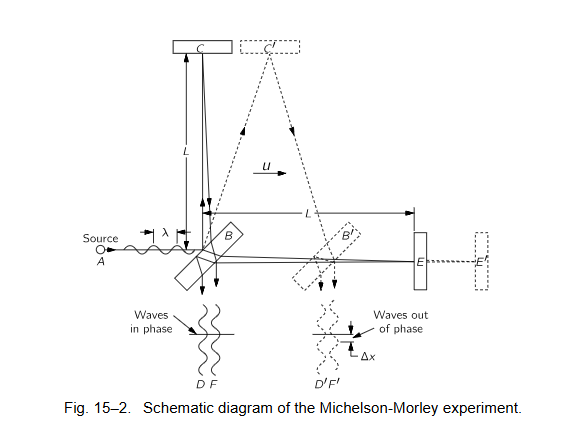
\includegraphics[width=0.8\textwidth]{Michelson-Morley.png}
    \caption{Diagram from Feynman's lecture notes}
\end{figure}
When they're at rest, since the distance $L$ are equal light takes the same time to go from $B$ to $C$ and back as it takes to go from $B$ to $E$ and back, so when the two rays meet they interfere constructively. However, when the mirrors move together with velocity $u$ (preserving the distances) the times differ, then the relative velocity of the light is $c-u$, and let $t_{BE}$ be time $B \rightarrow E$.
\[
t_{BE} = \frac{L}{c-u}
\]
The returning time can be calculated similarly.
\[
t_{EB} = \frac{L}{c+u}
\]
So the total time is the sum.
\[
t_{//} = t_{BE} + t_{EB} = \frac{2Lc \xcancel{+Lu - Lu}}{c^2 - u^2} = \frac{2L/c}{1 - u^2/c^2}
\]
Notice that the nominator $\frac{2L}{c}$ is just the time if the system is at rest.

Now to calculate the times $t_{BC}$ and $t_{CB}$ observe that light moves along the hypotenuse of a triangle with height $L$ and base length $ut_{BC}$.
\[
(ct_{BC})^2 = L^2 + (ut_{BC})^2
\]
Which simplifies to the following.
\[
t_{BC} = \frac{L}{\sqrt{c^2 - u^2}}
\]
Notice that due to the symmetry of the distances $t_{BC} = t_{CB}$.
\[
t_{\perp} = t_{BC} + t_{CB} = \frac{2L}{\sqrt{c^2 - u^2}} = \frac{2L/c}{\sqrt{1 - u^2/c^2}}
\]
As we can see the time taken by the light moving in each direction isn't equal, which means it can interfere destructively and we can measure the $u$ using that information. But when this was attempted experimentally the velocity of earth was calculated to be zero! Because no time difference was found.

Lorentz found that a moving body must contract in the direction parallel to its motion to correct that falsely predicted time difference, by substituting $L_{//} = \sqrt{1-\frac{u^2}{c^2}} \cdot L$ we can equate the traveling times.
\[
t_{//} = \frac{2L/c}{1 - u^2/c^2} \cdot \sqrt{1-\frac{u^2}{c^2}} = \frac{2L/c}{\sqrt{1 - u^2/c^2}} = t_{\perp}
\]

We can see from this that a moving body must contract to produce the observed lack of time difference.

Physicists found that Maxwell's equations \emph{are} correct and the speed of light \emph{is} constant. Then Poincare and Einstein concluded that it isn't constant relative to the hypothetical ether, it's absolutely constant in every frame of reference. And that any physical law which allows an observer with constant velocity to measure their velocity must be corrected.

\section*{Time Dilation}
In the previous experiment you may have noticed that in a moving system light takes a longer time to reflect back than in a stationary system. So if an observer is able to perceive time they may be able to measure their velocity using that information.
\begin{figure}[htbp]
    \centering
    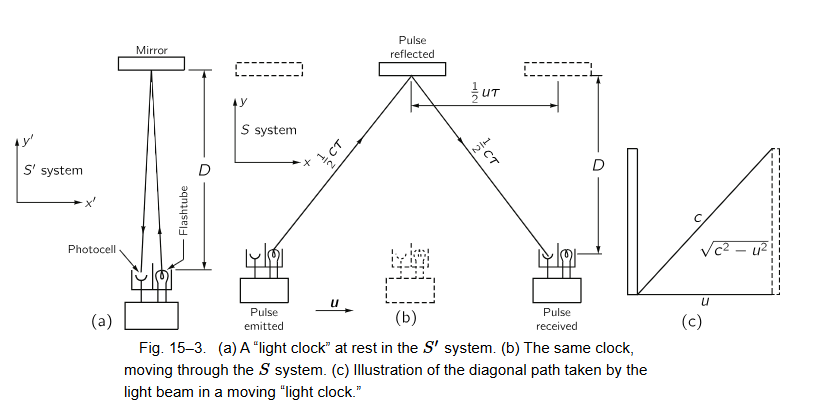
\includegraphics[width=0.9\textwidth]{Light-Clock.png}
\end{figure}

\end{document}
